\chapter{Reti Neurali}
\label{chap:RetiNeurali}

Nel campo dell'apprendimento automatico (o machine learning), una rete neurale artificiale (\textbf{ANN} "Artificial Neural Network") è un modello matematico basato sulla semplificazione delle reti neurali biologiche \cite{samuel1959some}. \\
Una rete neurale può essere considerata come un sistema dinamico avente la topologia di un grafo orientato con nodi (i neuroni artificiali) ed archi (pesi sinaptici).
Questo modello è composto da un gruppo di interconnessioni di informazioni costituite da neuroni artificiali che modellano i neuroni in un cervello biologico e processi che utilizzano un approccio di connessionismo di calcolo.
Ogni connessione, come le sinapsi di un cervello biologico, può trasmettere un segnale da un neurone artificiale a un altro, i quali sono tipicamente aggregati in strati. 
Gli stimoli vengono ricevuti da un livello di nodi d'ingresso detto unità di elaborazione. Il neurone artificiale che riceve il segnale può elaborarlo e quindi trasmetterlo ad altri neuroni artificiali collegati ad esso.\\
Poiché nell'implementazione di ANN tradizionali i segnali vengono rappresentati da numeri reali, possiamo considerare questa elaborazione come una moltiplicazione tra gli ingressi e un valore detto peso. Il risultato di queste operazioni viene sommato e se la somma supera un certa soglia il neurone si attiva, attivando la sua uscita.
Il peso serve a quantificare l'importanza dell'efficacia sinaptica della linea di ingresso.		\\
Sono strutture non-lineari di dati statistici e vengono utilizzate per simulare relazioni complesse tra ingressi ed uscite che altre funzioni analitiche non sono in grado di rappresentare.\\

\begin{figure}
	\centering
	{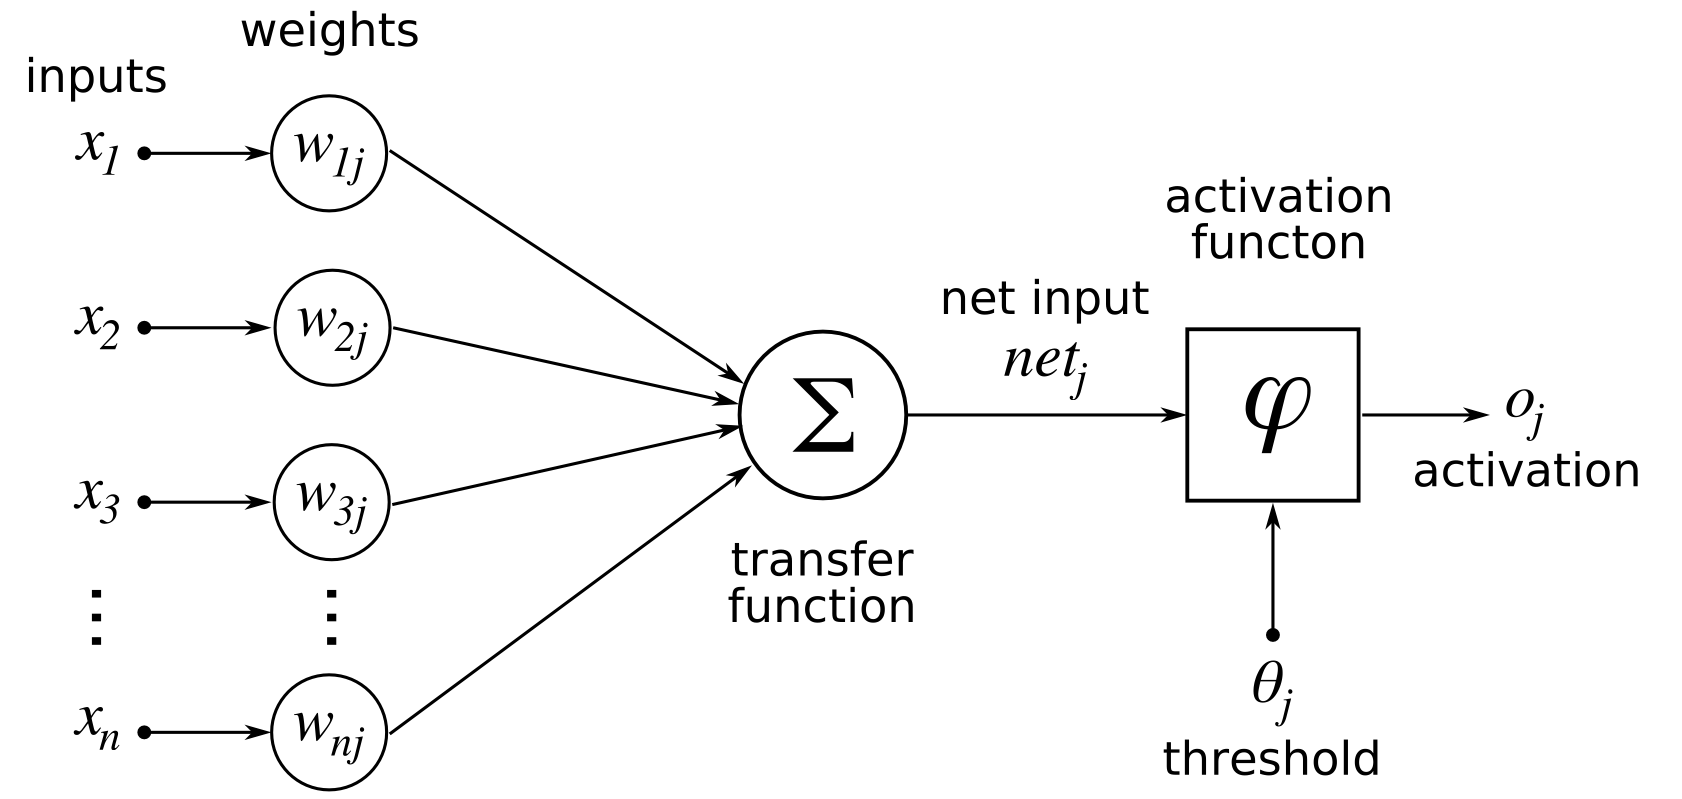
\includegraphics[width=.65\textwidth]{images/ArtificialNeuronModel}} \quad
	\caption{Artificial Neuron Model}
	\label{fig:Artificial Neuron Model}
\end{figure}

\section{Definizioni}
\label{sec:def}
Le reti neurali possono essere viste come semplici modelli matematici che definiscono una funzione $f:X\rightarrow Y$. \\
La funzione di rete di un neurone $f(x)$ è definita come una composizione di altre funzioni $g_i(x)$, che possono a loro volta essere scomposte in altre funzioni. Questo può essere rappresentato come una struttura di reti.\\
Una rappresentazione ampiamente utilizzata è la \emph{somma ponderata non lineare}, dove 
\begin{equation}
f(x)=K \bigg( \sum_{i}w_ig_i(x)\bigg)
\end{equation}
dove $k$ è una funzione predefinita, detta anche \emph{funzione di attivazione}.
\\\\
Ad ogni input $x_i$ è associato un peso $w_i$ con valore positivo o negativo per eccitare o inibire il neurone. Il bias varia secondo la propensione del neurone ad attivarsi, per variare la soglia di attivazione del neurone.
Secondo l'algoritmo, dopo il caricamento dei valori di input e i pesi relativi, si prosegue calcolando la somma dei valori di input pesata con i relativi pesi. In seguito viene calcolato il valore della funzione di attivazione $K$ con il risultato della somma pesata.
L'output del neurone $y$ è il risultato ottenuto dalla funzione di attivazione
\begin{equation}
y(x)=K\bigg( \sum_{i=1}^{d}w_ix_i+w_0\bigg) = \overline{w}^T\overline{x}
\end{equation}

\subsection{Funzione di attivazione}
\label{subsec:fattivazione}
La funzione di attivazione di un nodo determina la risposta di quel neurone.\\
Solo le funzioni di attivazione non lineare consentono a tali reti di calcolare problemi non banali utilizzando un  numero limitato di nodi.\\\\
Utilizzando una funzione di attivazione Sigmoide normalizzabile, il modello realistico rimane a zero fino a quando viene ricevuta la corrente di ingresso, a quel punto la frequenza di accensione aumenta rapidamente all'inizio, ma gradualmente si avvicina a un asintoto con una frequenza di attivazione del 100\% \cite{han1995influence}.

\begin{equation}
f (x) = \frac{1}{1+e^{-x}}
\end{equation}
$\\$
Un'altra delle funzioni di attivazione più utilizzate è la ReLU (Rectified Linear Unit) \cite{nair2010rectified}, definita dalla seguente 
\begin{equation}
f (x) = max(0, x)
\end{equation}
Questa funzione semplicemente setta a zero tutti i valori negativi, mentre ritorna lo stesso valore per quelli positivi.
La ReLU viene utilizzata in quanto rende più rapido ridurre l’accuratezza ed inoltre risolve parzialmente il problema del "vanishing gradient" che porta i layer più in profondità della rete ad imparare troppo lentamente.


\begin{figure}
	\centering
	\subfloat[][\emph{Sigmoide}]
	{\includegraphics[width=.45\textwidth]{images/signmoid2}}
	\quad
	\subfloat[][\emph{ReLU}]
	{\includegraphics[width=.45\textwidth]{images/relu2}} 
	
	\caption{Funzioni di attivazione}
	\label{fig:subfig}
\end{figure}



\section{Apprendimento}
\label{sec:apprendimento}
Per insegnare alla rete a risolvere il problema occorre un periodo di apprendimento in cui vengono sfruttate una serie di osservazioni per trovare ciò che risolvere il compito in maniera ottimale. \\
Questo comporta la definizione di una \emph{funzione di costo} in grado di misurare la distanza tra una soluzione particolare ed una ottimale per il problema. Gli algoritmi di apprendimento cercano una funzione che abbia il minor costo possibile.\\
La conoscenza estratta dalla rete viene memorizzata sui pesi che vengono modificati sfruttando tecniche di ottimizzazione. \\\\
La funzione di errore è l'espressione della differenza/scostamento tra l'output della rete $y$ e l'output desiderato $y'$ nell'apprendimento
\begin{equation}
E(w)=\sum_{i=1}^{c}((y_i-y'_i)^2)
\end{equation}


{\color{blue}
	\subsection{Algoritmo di back propagation}
	\label{subsec:backprop}}

\subsection{Paradigmi di apprendimento}
\label{subsec:Paradigmi di apprendimento}

Gli algoritmi di apprendimento sono principalmente suddivisi in due categorie:
\begin{itemize}
	\item[\bfseries supervisionato] --- alla rete viene presentato un training set preparato da un "insegnante esterno", composto da coppie significative di valori (input, output atteso/desiderato).\\
	Quando alla rete neurale viene fornito l'input dall'ambiente, l'insegnante è in grado di calcolare/restituire l'output desiderato corrispondente addestrando la rete mediante un algoritmo (tipicamente quello di back propagation). 
	Durante questo procedimento viene calcolo l'errore che la rete commette, necessario per farle comprendere di quanto sbaglia ed è dato dalla differenza tra l'output e l'output atteso. La rete modifica i propri pesi in base all'errore commesso, che rappresenta l'azione ottima per l'input corrente, cercando di minimizzarlo.\\
	In questo moto la rete impara a riconoscere la relazione incognita che lega le variabili di ingresso e uscita, in modo da prevedere il valore di output per qualsiasi valore di ingresso, basandosi solo su una limitata casistica di corrispondenza (coppie input-output).
	
	\item[\bfseries non supervisionato] --- alla rete vengono presentati solo i valori di input, mentre non sono messe a disposizione le informazioni di ritorno dell'ambiente sui valori obiettivo che si vogliono ottenere in risposta o riguardo la correttezza dell'output fornito. \\
	La rete individua da sola pattern, caratteristiche, similarità e regolarità statistiche nei dati di input, acquisendo la capacità di dividerli in cluster rappresentativi in modo da sviluppare delle rappresentazioni interne, senza usare confronti con output noti.\\ 
	In questo caso gli algoritmi che modificano i pesi della rete fanno riferimento solo ai dati contenuti nelle variabili di ingresso.\\
	Questo è un tipo di apprendimento autonomo e non c'è controllo esterno sull'errore. Adatto per ottimizzare risorse e se non si conoscono a priori i gruppi in cui dividere l'input.
\end{itemize}


%\subsection{Tasso di apprendimento}
%\label{subsec:learnrate}
%modificando i valori dei pesi dopo ogni presentazione di una configurazione dell'input invece che dopo la presentazione di un ciclo completo di configurazioni, realizza una discesa nello spazio dei pesi che non è necessariamente la più ripida. È comunque corretto approssimare tale discesa alla più ripida purché ad ogni passo del processo iterativo di apprendimento i pesi non vengano modificati di quantità troppo grandi, fissando un tasso di apprendimento $\mu$ piccolo.\\
%Il processo di discesa del gradiente può essere estremamente lento se il valore del tasso di apprendimento $\mu$ è troppo piccolo; d'altra parte, valori troppo elevati di  $\mu$ introducono fenomeni di oscillazioni durante la discesa. Il problema delle oscillazioni è fortemente legato alla presenza di valli profonde con pendenza quasi nulla sul fondo della superficie della funzione errore; in questi casi il vettore dei pesi ad ogni aggiornamento presenta una componente diretta verso il punto di minimo della funzione errore, ma anche una componente che lo devia da tale direzione e che è la causa di oscillazioni che hanno direzione opposta in aggiornamenti consecutivi. \\
%


\section{Development and test set }
\label{sec:DevelopmentAndTestSet}
Per misurare le prestazioni di una rete neurale dopo la fase di apprendimento, viene creato un test set formato da coppie non utilizzate per il training e validation set.\\
Vengono generalmente definiti: 
\begin{itemize}
	\item Training set – Sul quale viene eseguito l'algoritmo di apprendimento.
	\item Dev (development) set – Viene utilizzato per regolare i parametri, selezionare le features e prendere decisioni per quanto riguarda l'algoritmo di apprendimento. Talvolta viene anche chiamato set di hold-out / cross  validation. (convalida incrociata)
	\item Test set – si utilizza per valutare le performance/prestazioni dell'algoritmo, ma non per prendere decisioni su quale algoritmo di apprendimento o parametri utilizzare. 
\end{itemize}

Una volta definiti i set di development e test, ci si concentrerà sul miglioramento delle prestazioni del development set. \\
Generalmente la dimensione di del test set è un terzo del training set, ed è composto da input critici su cui la risposta della rete deve essere buona.
Questo funziona bene quando sono messi a disposizione un numero limitato di esempi, ma nell'era dei big data, dove i problemi di apprendimento automatico consistono di più di un miliardo di esempi, la frazione di dati allocati agli insiemi di sviluppo / test è ridotta, nonostante il valore assoluto di esempi sia aumentato/maggiore.\\
Vengono utilizzate diverse tecniche statistiche per valutare la bontà nella rete. Normalmente si accetta una rete se sul test set viene mostrato un errore inferiore al 20-25\%.



\subsection{Evaluation metric}
\label{subsec:EvaluationMetric}
La \emph{precisione} di classificazione è un esempio di una metrica di valutazione di un singolo numero: si esegue il classificatore sul set di sviluppo (o set di test) e si ottiene un numero singolo su quale frazione di esempi è stata classificata correttamente. Secondo questa metrica, se il classificatore A ottiene l'accuratezza del 97\%, e il classificatore B ottiene l'accuratezza del 90\%, allora giudichiamo che il classificatore A sia superiore.\\ 
Al contrario la \emph{recall} non è una singola metrica di valutazione numerica: due numeri per la valutazione del classificatore. Avere metriche di valutazione a più numeri rende più difficile confrontare gli algoritmi.
\\
Avere una singola metrica di valutazione del numero come l'\emph{accuratezza} consente di ordinare i modelli in base alle loro prestazioni su questa metrica e decidere rapidamente che cosa funziona meglio.

\subsection{Overfitting}
\label{subsec:overfitting}

L'\emph{overfitting} è "la produzione di un'analisi che corrisponde troppo o esattamente a un particolare insieme di dati, e può quindi non riuscire ad adattare dati aggiuntivi o prevedere in modo affidabile le osservazioni future".\\
La rete neurale deve avere capacità di comprensione del modello statistico dei dati, non memorizzare i soli dati del training set. L'essenza del sovraffollamento consiste nell'estrarre inconsapevolmente parte della variazione residua (cioè il rumore) come se quella variazione rappresentasse la sottostante struttura del modello \cite{burnham2003model}.\\
Per ridurre la possibilità di overfitting esistono diverse tecniche come la convalida incrociata (cross validation), la regolarizzazione o l'\emph{early stopping}, che consiste nell'utilizzo di un validation set di coppie non usate nel training set per la misurazione dell'errore.\\
La base di alcune tecniche è per penalizzare esplicitamente i modelli eccessivamente complessi per testare la capacità del modello di generalizzare, valutando le sue prestazioni su un insieme di dati non utilizzati per l'addestramento.

\section{Reti neurali per la classificazione}
\label{sec:classificazione}
La classificazione è la suddivisione di oggetti in insiemi disgiunti secondo un criterio stabilito a priori (etichetta). Ogni oggetto viene rappresentato come un vettore di numeri in modo da poter essere classificato dalla rete neurale, un vettore di feature che contraddistingue univocamente el'oggetto.\\
\subsection{Definizione}
\label{subsec:defclass}
Date $N$ classi di appartenenza tra cui discriminare, il vettore di input $x$ possiede $L$ dimensioni delle feature da classificare, il vettore $y$ individua la classe formata da $N$ valori. Il classificatore riceve in input il vettore $x$ e restituisce in uscita il vettore $y$ dove $y_i=1$ se l'oggetto con l'input $x$ appartiene alla classe $i$ e $y_j=0$ per $i\neq j$ per $i,j=1 \dots N$.\\
Questo corrisponde ad una mappatura tra i valori di input e di output, che può essere modellata come una funzione non lineare.

\section{Reti neurali convoluzionali}
\label{sec:cnn}
Una rete neurale convoluzionale (o CNN "Convolutional Neural Network") è una classe di reti artificiali avanzate e \emph{feed-forward}, composte da uno o più strati convoluzionali con livelli completamente connessi (corrispondenti a quelli tipici di ANN) \cite{kim2014convolutional}. Questa architettura consente ai CNN di sfruttare la struttura 2D dei dati di input.\\\\
Una convoluzione può essere considerata come una funzione a finestra scorrevole, detta \emph{kernel} o filtro, applicata a una matrice. 
Nell CNN usiamo le convoluzioni sul livello di input per calcolare l'output. Ciò si traduce in connessioni locali, in cui ogni regione dell'ingresso è collegata a un neurone nell'output. Ogni livello applica filtri diversi, in genere centinaia o migliaia, e combina i loro risultati. Durante la fase di addestramento, una CNN impara automaticamente i valori dei suoi filtri in base all'attività che si desidera eseguire. \\
Le CNN sono adatte per elaborare dati visivi e altri dati bidimensionali. Hanno mostrato risultati superiori in entrambe le applicazioni di immagine e parlato. Possono essere addestrati con back-propagation standard. Le CNN sono più facili da addestrare rispetto ad altre reti neurali regolari, profonde e feed-forward e hanno molti meno parametri da stimare.\\
Una CNN è composta da un input e un livello di output, oltre a più livelli nascosti. Gli strati nascosti di una CNN consistono tipicamente di strati convoluzionali, strati di raggruppamento, strati completamente connessi e livelli di normalizzazione.\\
Rappresentano una delle tecniche più popolari nel campo del riconoscimento delle immagini ma anche nell'elaborazione del linguaggio naturale (NLP "Natuaral Language Processing") \cite{manning1999foundations,FIXME}.\\
In quest'ultimo caso, l'input sono frasi o documenti rappresentati come una matrice. Ogni riga della matrice corrisponde a un token, in genere una parola. Tipicamente, questi vettori sono dei word embeddings (rappresentazioni a bassa dimensione) come word2vec \cite{mikolov2013distributed} o GloVe \cite{pennington2014glove}, ma potrebbero anche essere vettori unici che indicizzano la parola in un vocabolario. Nel NLP utilizziamo filtri che scorrono su righe complete della matrice (parole). Pertanto, la "larghezza" dei nostri filtri è solitamente uguale alla larghezza della matrice di input. L'altezza, o la dimensione della regione, può variare, ma le finestre tipicamente scorrono su 2-5 parole per volta. \\
Risulta che le CNN applicate ai problemi di NLP funzionino abbastanza bene, un esempio è il modello \emph{Bag of Words} che è stato l'approccio standard per anni e ha portato a risultati piuttosto buoni.
